% !TeX root = ../main.tex
\titlespacing{\chapter}{0cm}{-2cm}{0cm}
\chapter{方法與理論}
為實現本研究目的,過程需要採用之方法將於本篇介紹其方法與理論,而詳細的流程與遭遇阻礙的解決辦法將於第三章一一詳細介紹。在本研究的過程中主要使用三種不同光源分別使用於不同用途,本章節將介紹這些光源間的區別、使用時機及適合之擬合模型。接著說明運算過程所需使用到的光譜數據,從一張已經透過光譜晶片聚焦於影像感測器上而含有光譜訊息的影像,該如何一步一步轉換成光譜,並介紹所需使用到的方法與理論,並說明如何加速此轉換方法並化簡其轉換方程式的運算過程。
\par
影像轉換為光譜後,並非所有數據皆可以直接使用,當光譜數據含有過曝點或者或暗的情形時,此組光譜數據在分析上將會難以分析,當轉換後光譜存在過曝點時,會造成擬合數據不足而使得透過模型擬合找出的精確波峰將會有很大的誤差,而當轉換後光譜整體過暗時,在汞氬燈分析時會因為氬燈區強度平均偏低而與雜訊混合難以辨識,因此影像轉換為光譜數據後,需要進行亮度分析,並且透過循環調整影像感測器亮度直到光譜數據適合於數據分析,此一步驟稱為Auto Scaling,並於本篇介紹其理論。
\par
為達波長校正之目的,當已經獲取適合分析之影像光譜數據後,如何找到設定的目標波峰像素位置,便是波長校正的重點,本研究通過Hilbert Transform判別粗略波峰的像素位置,這些粗略的波峰位置雖然並非是最後所需的精確波峰結果,但對於去除無效的波峰提供大大的貢獻,粗略的波峰位置可以讓我們首先剃除與其差距過大的雜訊波峰。
\par
找出粗略波峰位置後,會對光譜數據進行數據分區,使每個區域中僅存在單一波峰,並在數據分區後透過模型擬合找出精確波峰。在本章將介紹Hilbert Transform理論與其特性,並介紹勞倫茲模型函數與高斯模型函數並說明如何後過數據點找出適合之模型參數。
\section{光源介紹}
本文於光譜晶片波長校正共採用三種不同光源,使用汞氬燈與雷射做於標準波峰的參考,並在校正結束後以白光LED\cite{White-LED}與汞氬燈之光譜做為晶片優劣的量化判別,此三種光源之產生方式、波長範圍與其適合的擬合模型列於表\ref{光源介紹表}. 中。

\begin{center}
\vspace{0.8cm}
\captionof{table}{光源介紹表}\label{光源介紹表}	
\begin{tabularx}{\textwidth}{|m{0.15\textwidth}<{\centering}|m{0.3\textwidth}<{\centering}|m{0.2\textwidth}<{\centering}|m{0.236\textwidth}<{\centering}|}
	\hline
	光源&產生方式 & 波長範圍(nm) & 適合之擬合模型\\		
	\hline
	汞氬燈&\multicolumn{1}{m{0.3\textwidth}|}{通過同時刺激汞原子與氬原子導致其電子躍遷釋放能量而產生光子束。}&253-922&勞倫茲模型\\
	\hline
	雷射&\multicolumn{1}{m{0.3\textwidth}|}{通過於共振腔中使用不同增益物值(gain media)將光線特定波長的能量放大。}&300-1200&勞倫茲模型\\
	\hline
	白光LED&\multicolumn{1}{m{0.3\textwidth}|}{以藍光LED激發黃色螢光粉使其產生白光,為兩波長合成之白光。}&400-900&\multicolumn{1}{m{0.236\textwidth}|}{需同時使用勞倫茲模型與高斯模型}\\
	\hline
\end{tabularx}
%\captionsetup{type=table}
\vspace{10pt}
\end{center}
\par
由表\ref{光源介紹表}. 中可以看出,用於波長校正上的雷射與汞氬燈光源,波段落於約250nm至1000nm之間,因此校正完之光譜晶片模組之有效應用區域約莫落於200nm至1200nm。電子躍遷\cite{42310}與藍光LED所產生之光束光譜逼近於勞倫茲函數\cite{Lorentz-1},而螢光激發之光束則接近於高斯函數。因汞氬燈為同時刺激汞與氬兩原子而產生電子躍遷釋放光束,因此兩光譜無法分開取出,造成校正上的困難,解決提案本文將於3.6.1節中詳細介紹。白光則因由藍光激發螢光產生由兩波長合成之白光,因此彼此之間相互影響,光束疊加區域造成模型擬合上的難題,本文將於3.8節詳細介紹。
\section{光譜影像轉換光譜}
光譜影像需將三通道影像之RGB參數透過轉換公式轉換為單通道灰度值,灰度則可視為光譜數據之光強度\cite{RGB-to-Spectrum}\cite{gray_as_Intensity},將所有像素點透過此種方式轉換為光度後,則可獲得影像之光譜數據,然而此種轉換方式運算量大,而且並非所有像素皆有義義,因此若將所有像素點皆轉換,會造成許多無意義多餘的運算,而造成效率低下,所以本節除了介紹影像轉換光譜的公式推導與理論外,也將介紹何謂興趣區間(Region of Interest, ROI),並會在第三章詳細介紹ROI的找尋方式。

\subsection{色彩轉換理論}
光源經過光譜晶片的分光等光學處理後聚焦於影像感測器上,則可獲得光源的光譜影像。當一白光光源透過光譜晶片處理距焦於感測器並且由影像感測器所取出$1280\times960$共含有122880個像素點的影像,如圖\ref{2.1,全幅光譜影像}. 所示。
\begin{figure}[H] %H为当前位置,!htb为忽略美学标准,htbp为浮动图形
	\centering %图片居中
	\vspace{0.8cm} 
	\setlength{\abovecaptionskip}{0.6cm}
	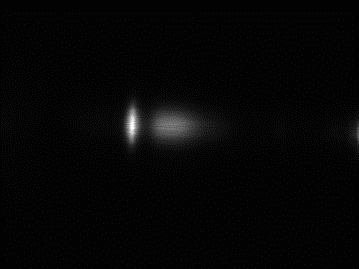
\includegraphics[width=8.8cm]{figures/p2-1.PNG} %插入图片,[]中设置图片大小,{}中是图片文件名
	\caption{全幅光譜影像} %最终文档中希望显示的图片标题
	\label{2.1,全幅光譜影像} %用于文内引用的标签
\end{figure}
圖像的像素對應於二維空間中一個特定的位置,而圖像的灰度值能表示出光的強度。圖\ref{2.1,全幅光譜影像}. 為三通道RGB彩色影像,透過灰階色彩轉換公式,則可將三通道轉為由灰度表示的單通道光度影像圖。轉換公式如式(\ref{eq:RBGtrans1})所示。
\begin{equation}
\label{eq:RBGtrans1}
Gray = R\times0.299 + G\times0.587 + B\times0.114
\end{equation}
為了提升程式運算速度,將三位精度浮點數算法縮放1000倍,修改為整數運算法
\begin{equation}
	\label{eq:RBGtrans2}
	Gray = (R\times299 + G\times587 + B\times114 + 500) / 1000
\end{equation}
整數運算雖提高運算速度,但在需要高精度的光譜分析時,使用位移運算法,即將公式(\ref{eq:RBGtrans2})中RGB的灰階轉換係數分別放大2的20次方倍,得到
\begin{equation}
	\label{eq:RBGtrans3}
	Gray = R\times313524.224 + G\times615514.112 + B\times119537.664
\end{equation}
將公式(\ref{eq:RBGtrans3})係數四捨五入成整數運算後得
\begin{equation}
	Gray = (R\times313524 + G\times615514 + B\times119538) >> 20
    \label{eq:2.4}
\end{equation}
其中$>>$為位元右移運算子,即將公式(\ref{eq:2.4})所求得結果轉換為二進制後向右位移二十位元,即可求得該像素灰階值。
\subsection{興趣區間(Region of Interest, ROI)}
一張全幅影像帶有所有光譜訊息,也伴隨著許多多餘的光譜訊息,若將全幅影像皆納入計算,則會造成運算量的大幅提升,且更容易受到環境光等因素的干擾,因此找出影像的興趣區間(ROI)為光譜分析的重要步驟之一。\par
假設一輸入全幅影像如圖\ref{2.1,全幅光譜影像}. 所示,將影像以縱向三等份後如圖\ref{2.2,全幅光譜影像縱向分區}. 所示,明顯可以看出圖\ref{2.2,全幅光譜影像縱向分區}. 中上下兩個無光區不帶有光譜訊息,而對於波長校正來說,ROI必需包含所有橫像素,並且以縱方向的光度平均值強弱為波長校正ROI的判定方式。
\begin{figure}[H] %H为当前位置,!htb为忽略美学标准,htbp为浮动图形
	\centering %图片居中
	\setlength{\abovecaptionskip}{0.6cm}
	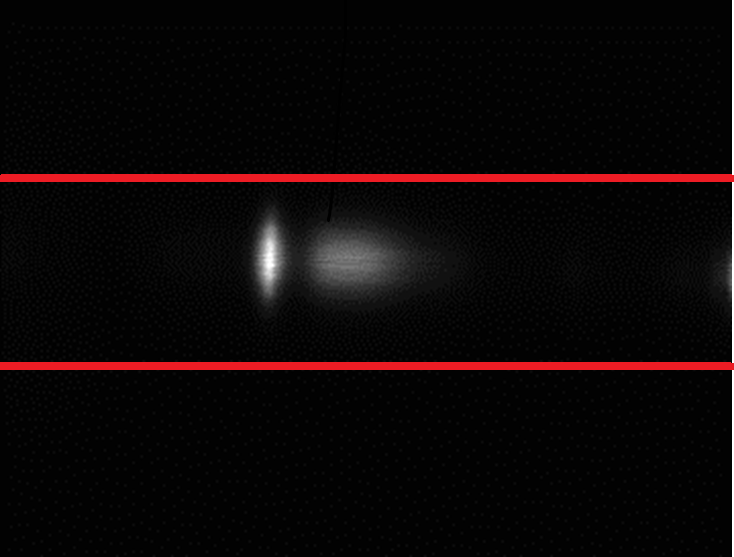
\includegraphics[width=8.8cm]{figures/p2-2.PNG} %插入图片,[]中设置图片大小,{}中是图片文件名
	\caption{全幅光譜影像縱向分區} %最终文档中希望显示的图片标题
	\label{2.2,全幅光譜影像縱向分區} %用于文内引用的标签
\end{figure}
\subsection{自動強度調整}
取出ROI光譜影像後,時常因影像感測器亮度參數過大、過小或光源強弱而導致影像無法分析。過曝影像之光譜會因其部份強度超過上限值,造成擬合參考點減少而計算出誤差極大的峰值位置,而過暗光譜影像之光譜會難以辨識雜訊與目標波峰,因此太弱或太高的強度都將導致後續分析處理的困難。
本文採用的影像感測器的可調參數分別為數位增益(Digital Gain, DG)、背光補償(Back Light, BL)與色差補償(Gamma)。各自的可調範圍顯示於表\ref{感測器參數}. 中。
\begin{center}
\vspace{0.8cm}
\captionof{table}{感測器參數範圍}\label{感測器參數}
\begin{tabularx}{\textwidth}{m{0.33\textwidth}<{\centering} m{0.33\textwidth}<{\centering} m{0.33\textwidth}<{\centering}}
	\hline\hline
	Name & Min & Max \\
	\hline
	DG & 32 & 255 \\
	\hline
	BL & 0 & 3\\
	\hline
	Gamma & 100 & 300 \\
	\hline\hline
\end{tabularx}
\vspace{10pt}
\end{center}
\par
由表\ref{感測器參數}. 可知,最適合細調的參數為DG\cite{DG},因其最小值與最大值差異最大且刻度最細,因此先固定其餘兩可變參數為最低值,再輸入不同的DG值獲得相對應的最大強度值I,將結果以數據組$(DG_i,I_i)$表示,又以知DG與光譜強度線性相關,故將兩組以上有效數據組直線擬合如圖\ref{DG與強度擬合結果圖}. 所示。
\begin{figure}[H] %H为当前位置,!htb为忽略美学标准,htbp为浮动图形
	\centering %图片居中
	\vspace{0.8cm}
	\setlength{\abovecaptionskip}{0.cm}
	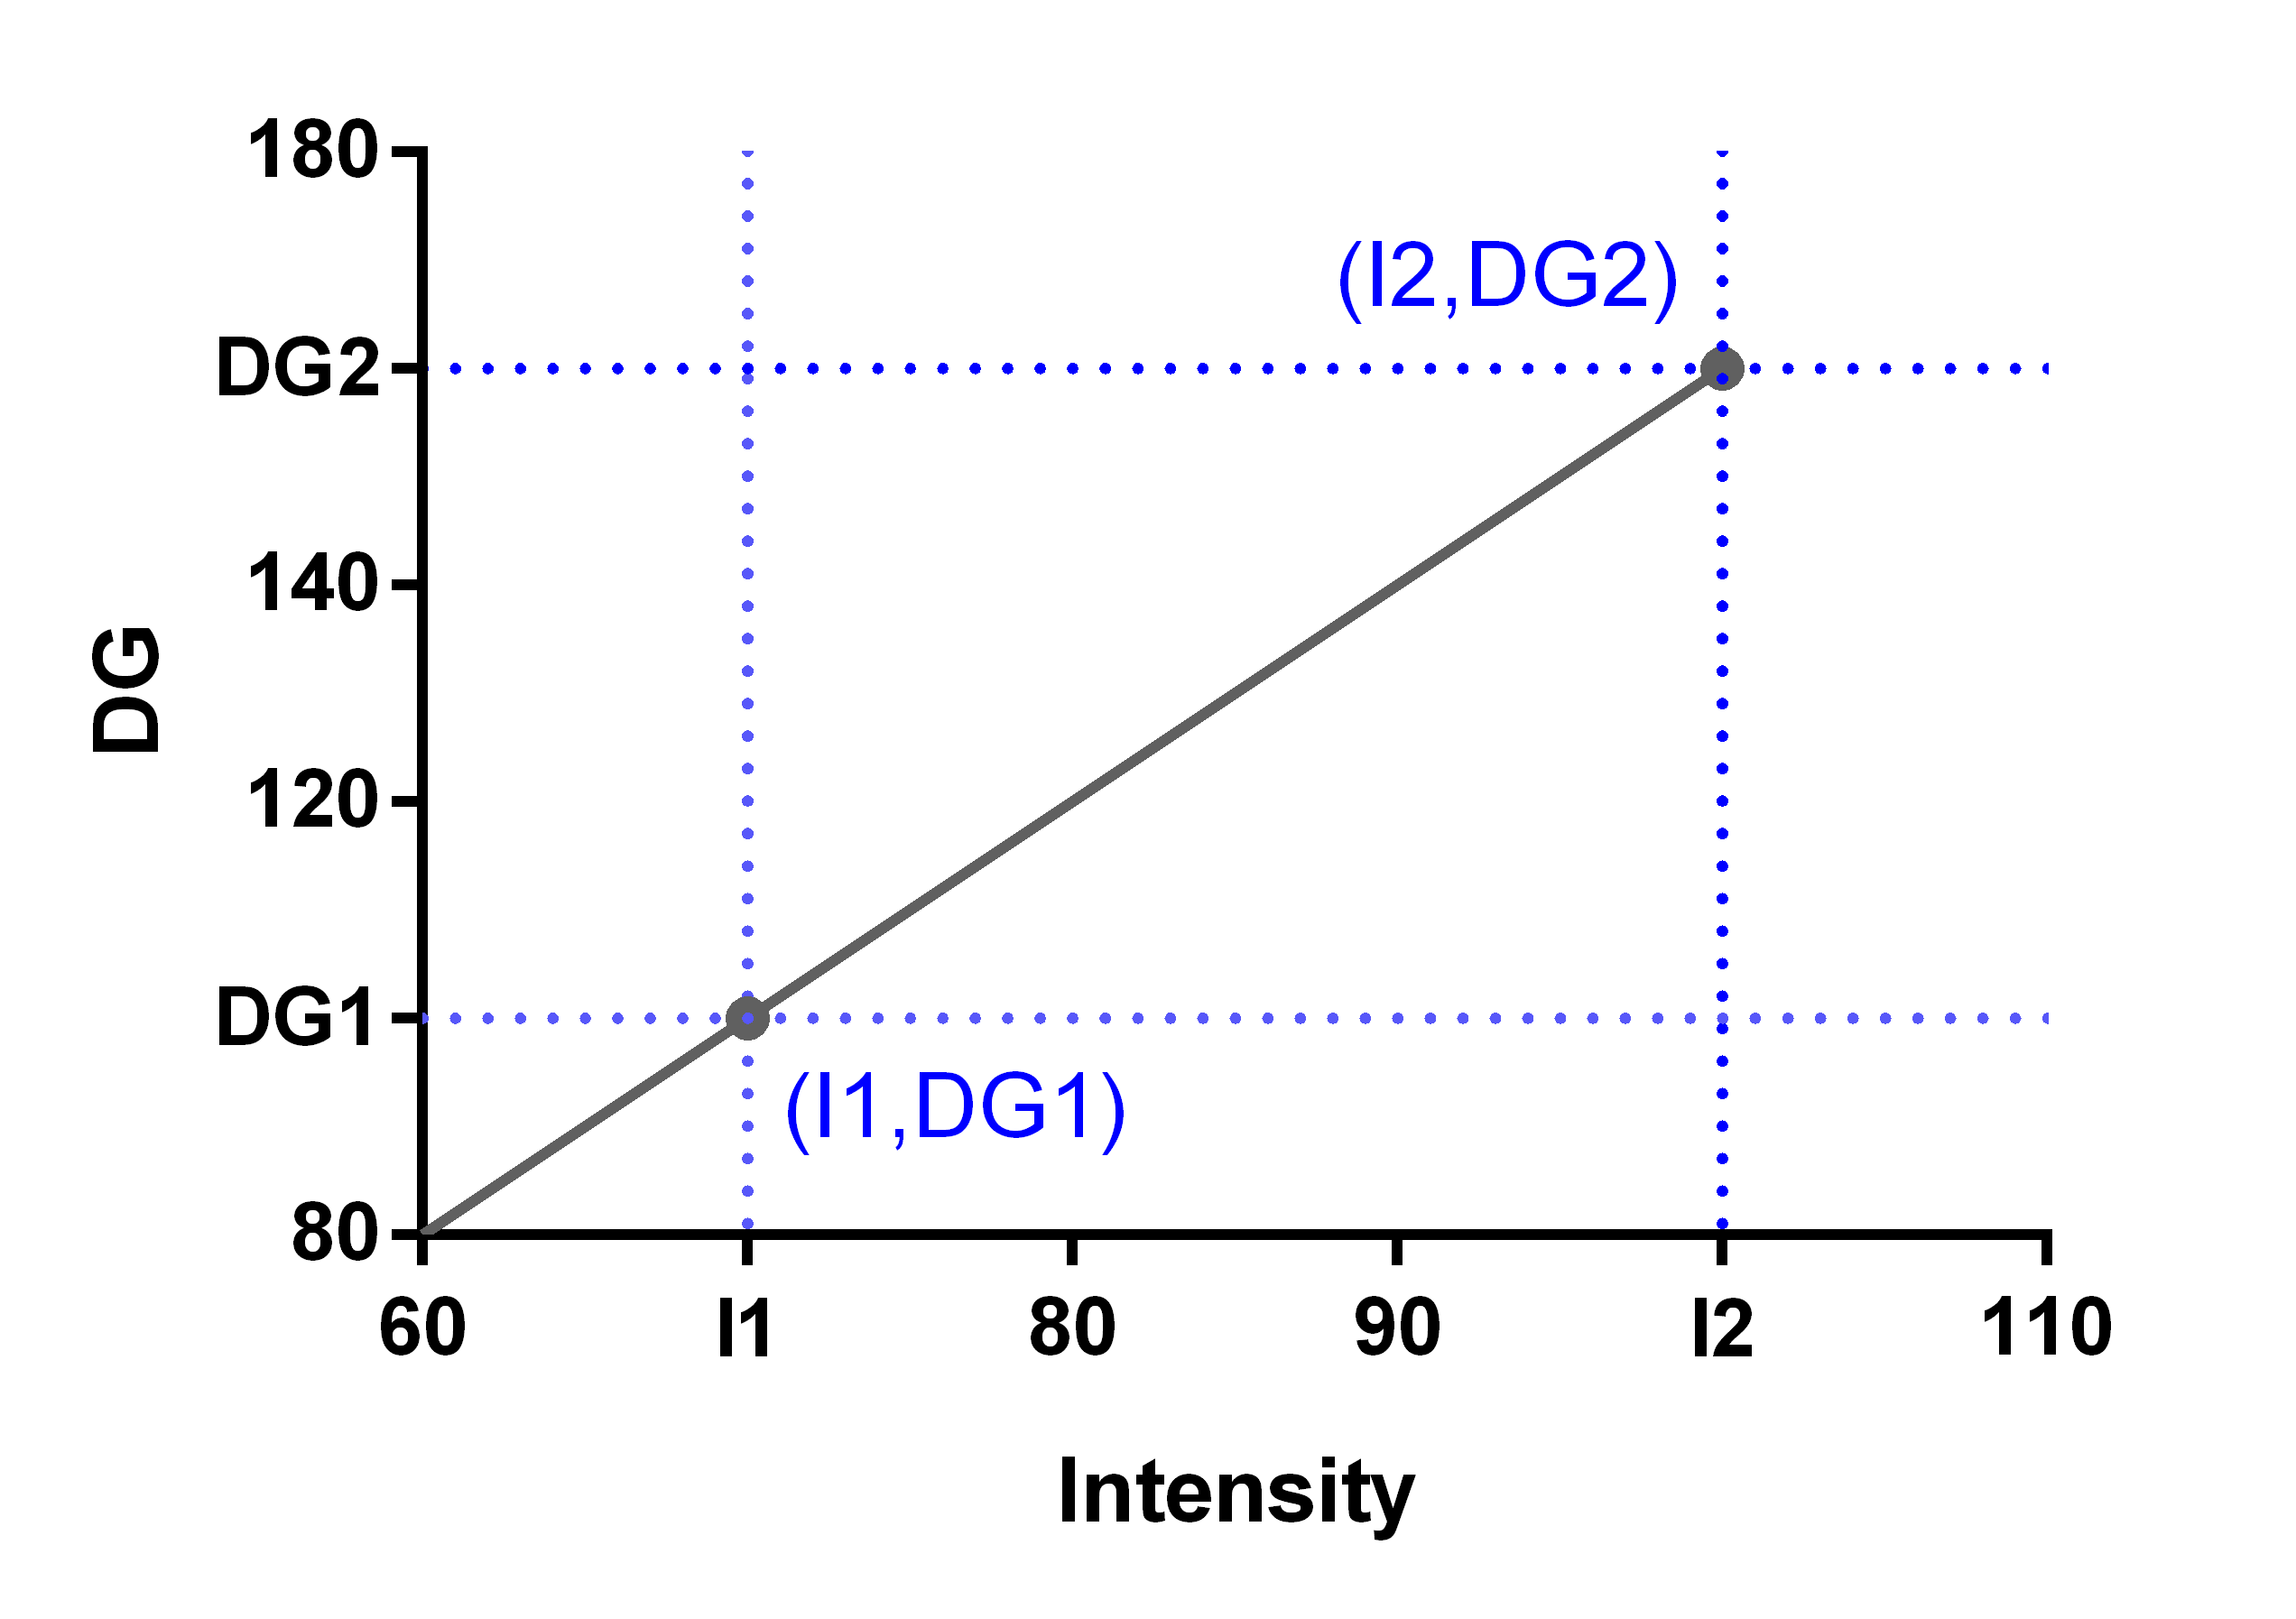
\includegraphics[width=13cm]{figures/AutoScaling.PNG} %插入图片,[]中设置图片大小,{}中是图片文件名
	\caption{DG與強度擬合結果圖} %最终文档中希望显示的图片标题
	\label{DG與強度擬合結果圖} %用于文内引用的标签
\end{figure}
今以數學式表示擬合直線為
\begin{equation}\label{eq:2.5}
	f(I) = aI+b\mid_{Gamma=100;BackLight=0}, \quad \forall a,b \in \mathbf{\mathbb{R}}
\end{equation}
由式(\ref{eq:2.5})可知,若欲將強度調整至$I_{max}$,則DG應設置為
\begin{equation}\label{eq:2.6}
	DG_{goal} = f(I_{max})\mid_{Gamma=100;BackLight=0}
\end{equation}
求出$DG_{goal}$並重新設置影像感測器參數後,即可獲得期望的最大強度值。
\section{Hilbert Transform運算}
在訊號理論中時常使用希爾伯特轉換(Hilbert Transform)\cite{Hilbert_book}估算粗略的信號峰值位置,本文中的峰值偵測演算法將利用Hilbert Transform找出粗略峰值像素位置並將信號分區。\par
一輸入訊號
\begin {math}
i(t) 
\end{math}
,與函數
\begin {math}
h(t) = \frac{1}{\pi t}
\end{math}
的卷積運算稱為Hilbert Transform,因此經Hilbert Transform後的輸出訊號表示為:
\begin{equation}\label{eq:2.7}
	y(t)=i(t)\ast h(t) = \frac{1}{\pi}\int_{-\infty}^{+\infty}i(t)\frac{1}{t-\tau}d\tau
\end{equation}
經由Hilbert Transform後的信號如圖\ref{單雷射波型經希爾伯特轉換}. 所示,輸入信號的峰值位置落在轉換後信號波谷與波峰的中心點,本文將此Hilbert Transform特性應用於3.5章波峰查找。
\begin{figure}[H] %H为当前位置,!htb为忽略美学标准,htbp为浮动图形
	\centering %图片居中
	\vspace{10pt}
	\setlength{\abovecaptionskip}{0.cm}
	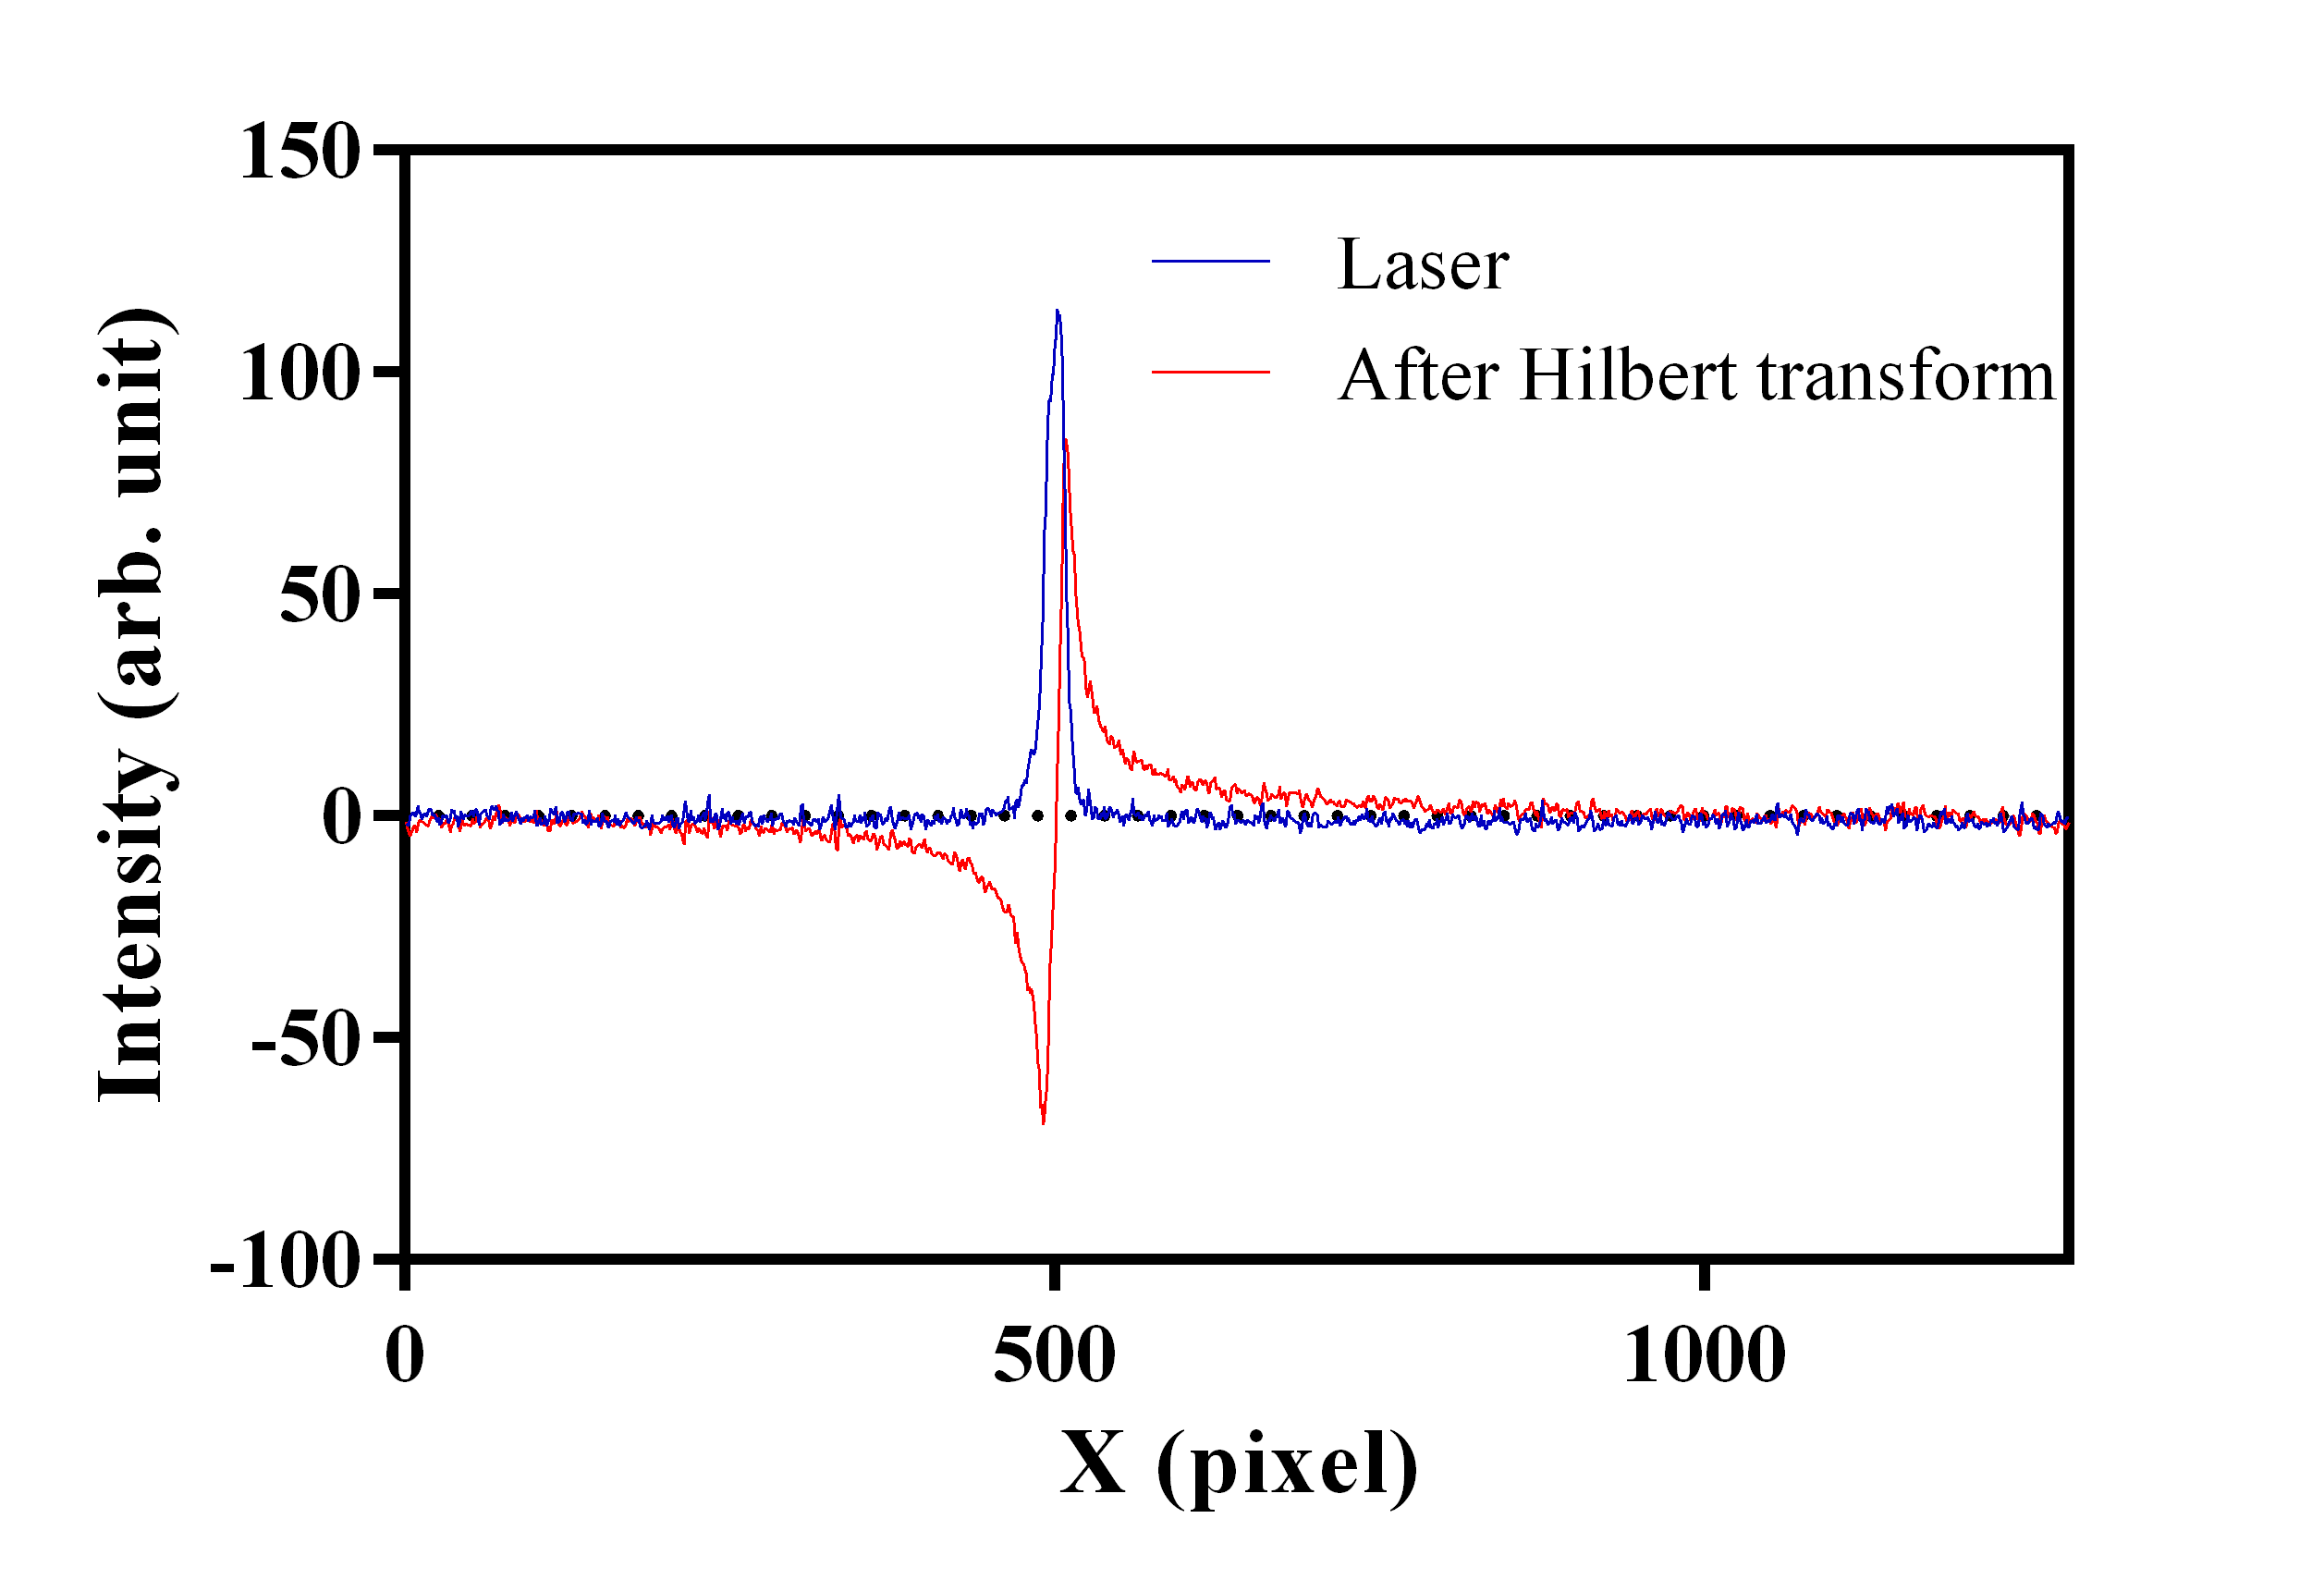
\includegraphics[width=16cm]{figures/p2-3_V2.png} %插入图片,[]中设置图片大小,{}中是图片文件名
	\caption{單雷射波型經Hilbert Transform轉換} %最终文档中希望显示的图片标题
	\label{單雷射波型經希爾伯特轉換} %用于文内引用的标签
\end{figure}
\section{光譜模型擬合}
光譜波形分析使用曲線擬合\cite{Spectral-fitting}的原因通常為分離不同波段光譜,但對於波長校正來說,使用曲線擬合的主要原因為以下兩點:
\par
	\textbf{一.} 光譜因環境光等眾多因素,導致波形失真,使用波形擬合可以將光譜逼近於完美波形,使光譜分析更加容易,圖\ref{雷射波形高斯擬合前後}. 為高斯擬合前後的結果對比。
	\begin{figure}[H]
		\centering
		\vspace{0.8cm}
		%\setlength{\belowcaptionskip}{-1cm} 
		\begin{subfigure}[fig nice]{0.49\textwidth}
			\setlength{\abovecaptionskip}{0.cm}
			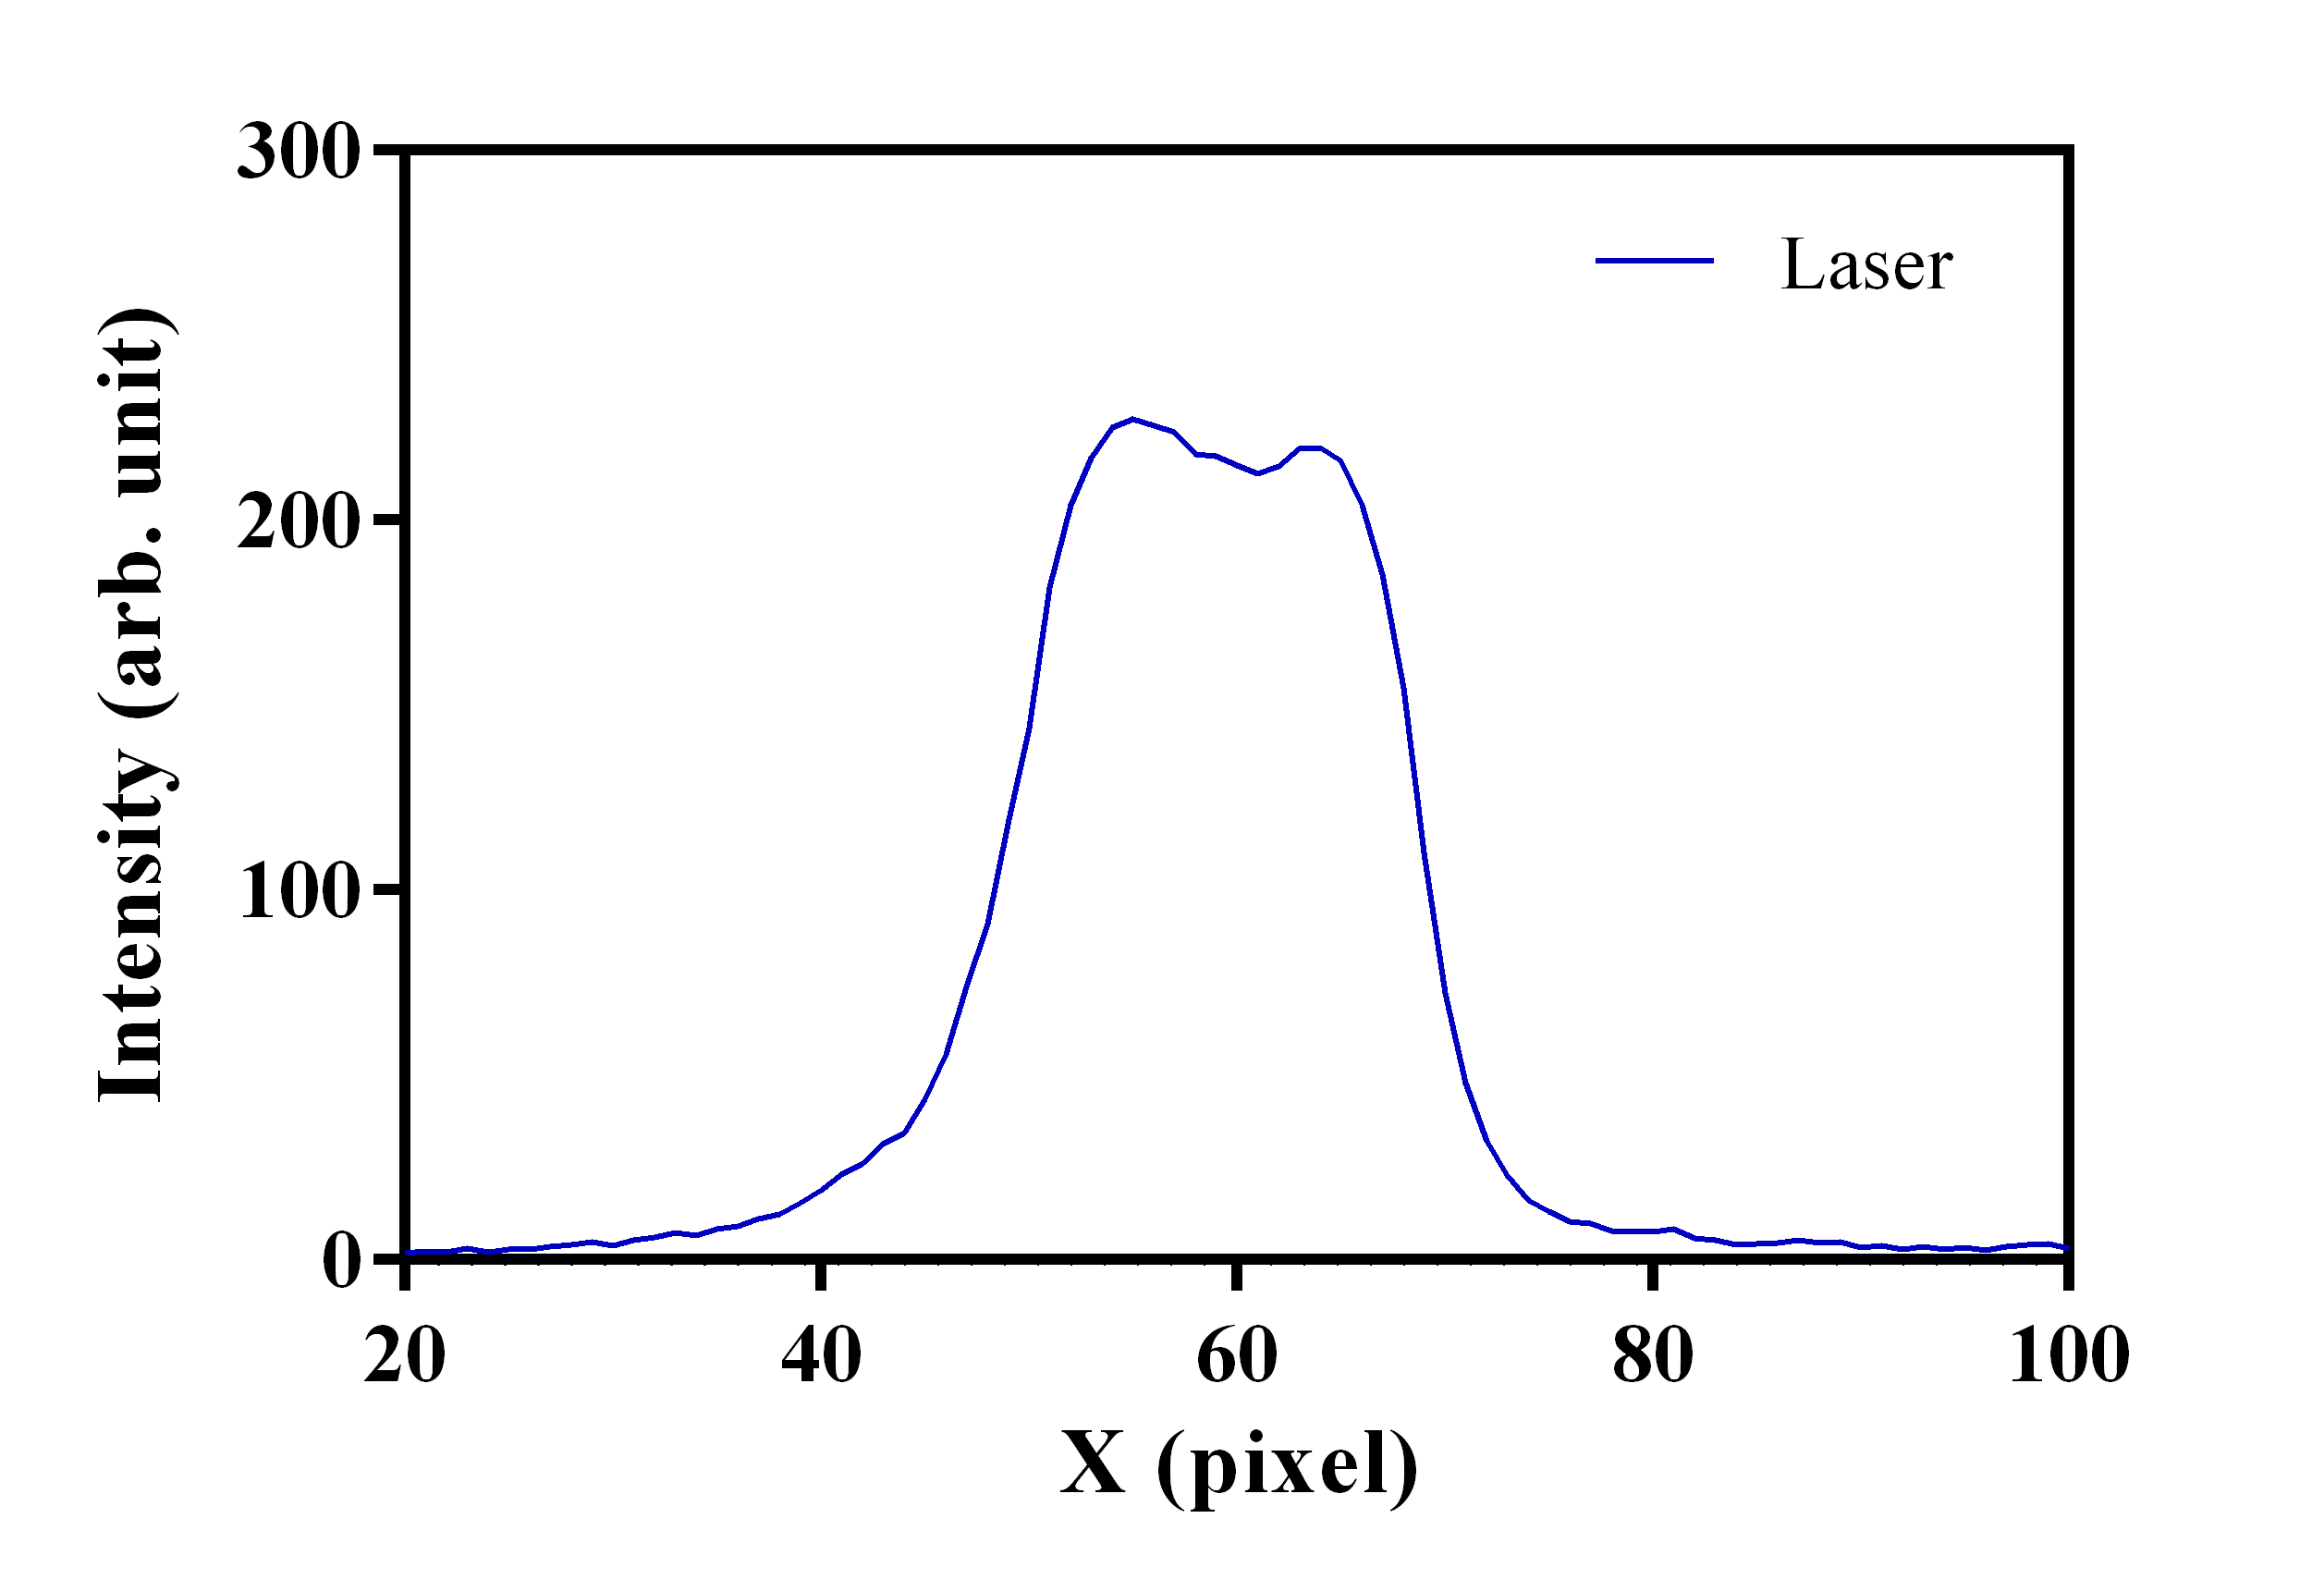
\includegraphics[width=7.9cm]{figures/Laser1.png}
			\caption{}
			%\subcaption{雷射波形}
			\label{雷射波形}
		\end{subfigure}
		\begin{subfigure}[fig nice]{0.49\textwidth}
			\setlength{\abovecaptionskip}{0.cm}
			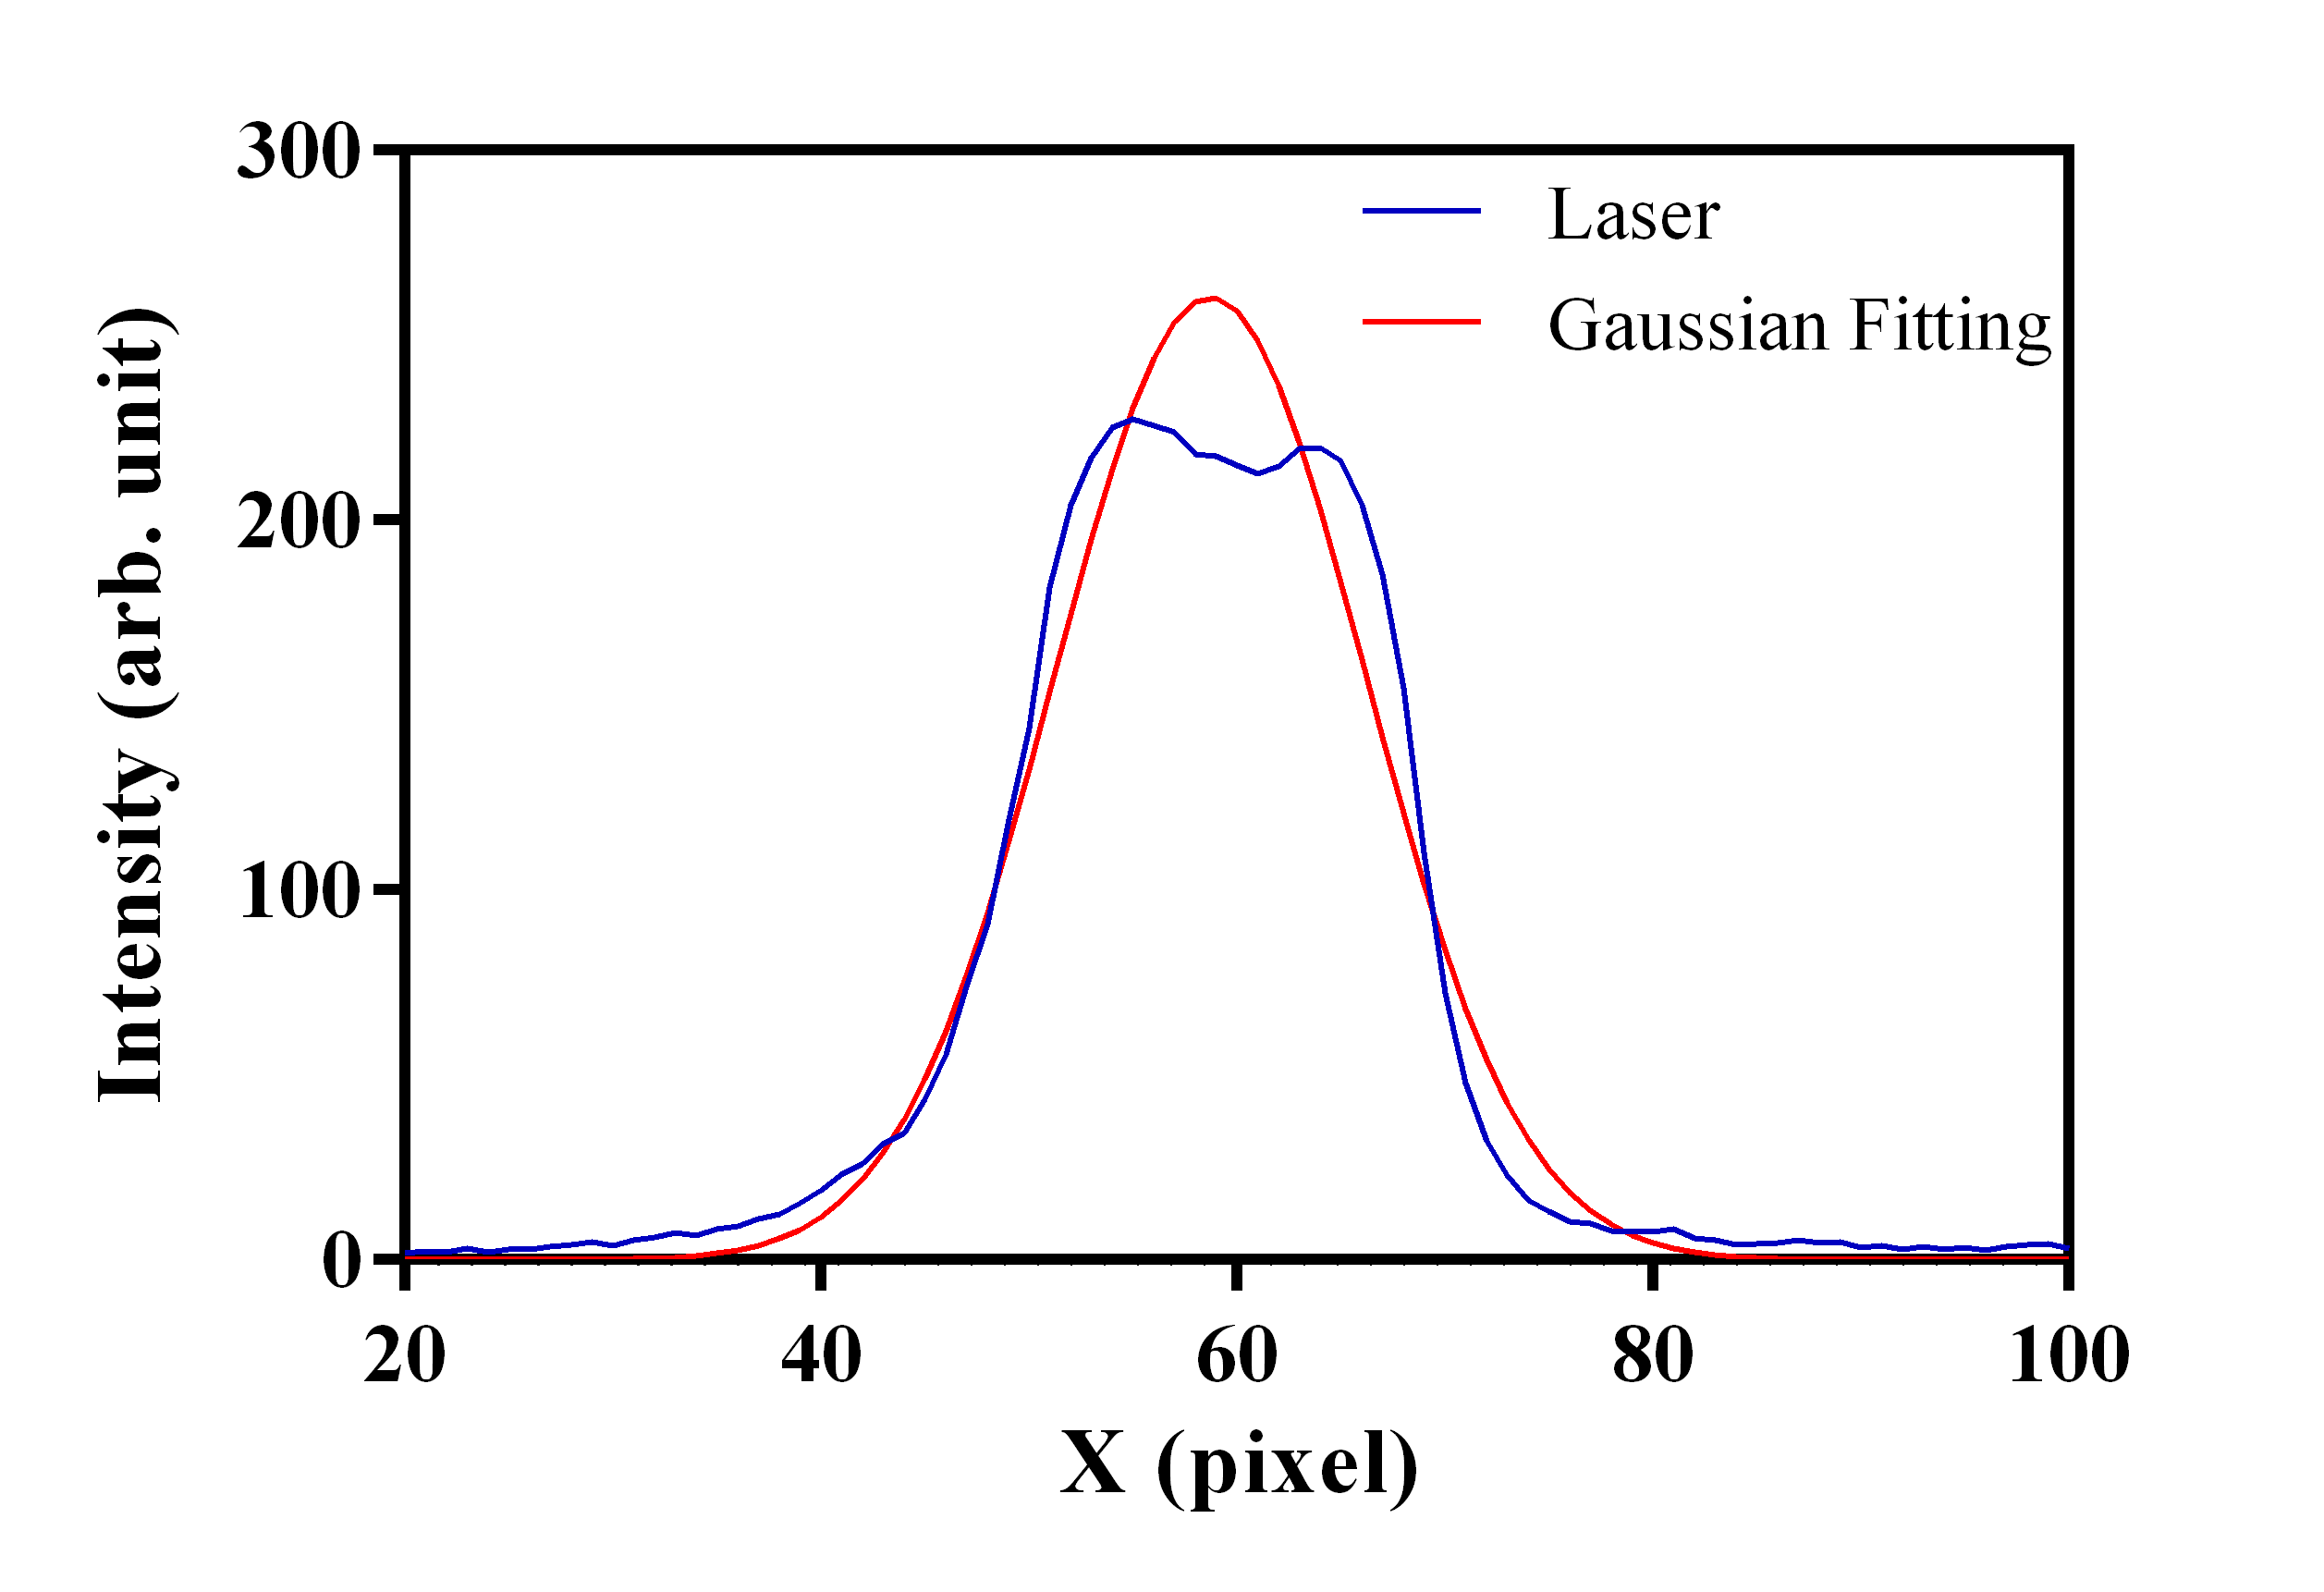
\includegraphics[width=7.9cm]{figures/Gassian_NEW600.png}
			\caption{}
			%\subcaption{高斯擬合後之雷射波形}
			\label{雷射經高斯擬合後}
		\end{subfigure}
	%\caption{雷射波形高斯擬合前後}
	\caption[失真嚴重的雷射波形高斯擬合前後比較圖]{雷射波形高斯擬合前後比較 (a)雷射原始波形(b)高斯擬合後之雷射波形}
	\label{雷射波形高斯擬合前後}
	\end{figure}
\textbf{二.} 當一光源進入影像感測器後,光源中心點受限於影像感測器像素值,無法精確表達出波峰正確位置。假設一完美無干擾光源波峰位置落在像素x = 404.35 pixel處,若單純由最高值方式偵測波峰,僅能找出x = 404 pixel,若採用波形擬合,可以利用其餘數據點加入模型擬合來找出最準確的波峰位置,表\ref{峰值位置比較表}. 顯示六束不同波長雷射的最大值位置與高斯擬合找出的最大值位置比較。
\begin{center}
\vspace{0.8cm}
\captionof{table}{峰值位置比較表}\label{峰值位置比較表}
\begin{tabularx}{\textwidth}{|c|m{1.5cm}<{\centering}|m{1.5cm}<{\centering}|m{1.5cm}<{\centering}|m{1.5cm}<{\centering}|m{1.41cm}<{\centering}|}
	\hline
	原始最大值位置(pixel)& 358 & 407 & 505 & 650 & 813\\
	\hline
	高斯擬合後最大值位置(pixel)& 357.69 & 406.85 & 504.52 & 650.26 & 812.72\\
	\hline
	誤差(pixel)&-0.31&-0.15&-0.48&0.26&-0.28\\
	\hline
\end{tabularx}
\vspace{10pt}
\end{center}

\subsection{高斯擬合}
高斯模型的函數\cite{Lorentz_AND_GAUSSIAN_book}形式為:
\begin{equation}\label{eq2.8}
	f(x)=a e^{\frac{-(x-b)^2}{2c^2}} \quad , \quad \forall a,b,c \in \mathbf{\mathbb{R}}
\end{equation}
今假設有一光譜數據組$(P_i,y_i)$其中$i=1,2,3,\cdots$欲使用高斯函數擬合,將此數據組以高斯函數描述:
\begin{equation}\label{eq2.9}
	y_i=y_{max} e^{\frac{-(P_i-P_{max})^2}{S}}
\end{equation}
其中的待估實數常數$y_{max}$、$P_{max}$與$S$分別代表高斯曲線的峰值、峰值位置與半高全寬訊息。將(\ref{eq2.9})
等號兩端取對數,化成:
\begin{equation}\label{eq2.10}
	\ln{y_i}=\ln{y_{max}}-\frac{(P_i-P_{max})^2}{S} = (\ln{y_{max}}-\frac{P_{max}^{2}}{S})+\frac{2P_i P_{max}}{S}-\frac{P_{i}^{2}}{S}
\end{equation}
令: 
\begin{equation}\label{eq2.11}
	\begin{cases}
		& \ln{y_i} = z_i \\
		& \ln{y_{max}}-\frac{P_{max}^{2}}{S} = b_0\\
		& \frac{2 P_{max}}{S} = b_1\\
		&  -\frac{1}{S} = b_2
		\end{cases}
\end{equation}\\
將(\ref{eq2.11})帶回(\ref{eq2.10})中替換,並以矩陣型式表示:
\\
\begin{equation}\label{eq2.12}
\begin{bmatrix} z_1\\z_2\\z_3\\ \vdots\\z_n\end{bmatrix} 
 \quad
= 
 \quad
 \begin{bmatrix} 
 	1&P_1&P_{1}^{2}\\
 	1&P_2&P_{2}^{2}\\
 	1&P_3&P_{3}^{2}\\
 	\vdots&\vdots&\vdots\\
 	1&P_n&P_{n}^{2}
 \end{bmatrix}
\begin{bmatrix} b_0\\b_1\\b_2 \end{bmatrix} 
\end{equation}
簡記(\ref{eq2.12})式為:
\begin{equation}\label{eq2.13}
  Z = PB
\end{equation}
則特徵參數矩陣$B$的最小二乘方解\cite{Least-Squart-method}為:
\begin{equation}\label{eq2.14}
	B = (P^TP)^{-1}P^T Z
\end{equation}
再根據式(\ref{eq2.11})求出$y_{max}$、$P_{max}$與$S$,即可求得高斯函數的峰值、峰值位置與半高全寬。

\subsection{勞倫茲擬合}
勞倫茲函數\cite{Lorentz_AND_GAUSSIAN_book}的函數形式為:
\begin{equation}\label{eq2.15}
	f(x)=\frac{I}{1+(\frac{x-p}{\gamma})^2}
\end{equation}
其中$I$為最大值,$p$為最大值位置,$\gamma$為半高全寬參數,其半高全寬為$2\gamma$,今假設有一組數據$(x_i,yi)$其中$i=1,2,3,\cdots$,欲以勞倫茲函數進行數據擬合,將數據組以勞倫茲函數表示:
\begin{equation}
	f_i= \frac{I_{max}}{1+(\frac{x_i-p_{0}}{\gamma})^2}
	\label{eq2.16}
\end{equation}
展開式(\ref{eq2.16})可得:
\begin{equation}\label{eq2.17}
	\frac{1}{f_i}= \frac{1}{I_{max}}(1+\frac{p_0^2}{\gamma^2})-\frac{2p_0}{I_{max}\gamma^2}x_i+\frac{1}{I_{max}\gamma^2}x_{i}^{2}
\end{equation}
令: 
\begin{equation}\label{eq2.18}
	\begin{cases}
		& \frac{1}{f_i} = z_i \\
		& \frac{1}{I_{max}}(1+\frac{p_0^2}{\gamma^2}) = b_0\\
		& -\frac{2p_0}{I_{max}\gamma^2} = b_1\\
		&  \frac{1}{I_{max}\gamma^2} = b_2
	\end{cases}
\end{equation}\\
將式(\ref{eq2.18})帶回(\ref{eq2.17})替換,並以矩陣表示為:
\\
\begin{equation}\label{eq2.19}
	\begin{bmatrix} z_1\\z_2\\z_3\\ \vdots\\z_n\end{bmatrix} 
	\quad
	= 
	\quad
	\begin{bmatrix} 
		1&x_1&x_{1}^{2}\\
		1&x_2&x_{2}^{2}\\
		1&x_3&x_{3}^{2}\\
		\vdots&\vdots&\vdots\\
		1&x_n&x_{n}^{2}
	\end{bmatrix}
	\begin{bmatrix} b_0\\b_1\\b_2 \end{bmatrix} 
\end{equation}
\\
簡記(\ref{eq2.19})式為:
\begin{equation}\label{eq2.20}
	Z = XB
\end{equation}
則特徵參數矩陣$B$的最小二乘方解為:
\begin{equation}\label{eq2.21}
	B = (X^TX)^{-1}X^T Z
\end{equation}
再將參數矩陣$B$之參數$b_0$、$b_1$與$b_2$帶回式(\ref{eq2.18})解聯立方程式得出$I_{max}$、$p_{0}$與$\gamma$。













